\documentclass[9pt]{beamer}
\usetheme{TUDOplain}
% workaround: provide commands not defiend by all bibtex styles
\providecommand{\btxandlong}{und}
\providecommand{\newblock}{}

\usepackage[english]{babel}
\usepackage[style=authortitle]{biblatex}
\addbibresource{../bibliography.bib}

% reformat footnotes very plain
\makeatletter
\renewcommand\@makefnmark{%
[\@thefnmark]}
\renewcommand\@makefntext[1]{%
  \noindent\tiny [\@thefnmark] #1}
\makeatother
% command for citing
\providecommand{\fcite}[1]{\footcite{#1}}
%

% basic utils
\usepackage[utf8]{inputenc}
\usepackage{enumerate}
\usepackage{graphicx}
\graphicspath{{../images/}}

\usepackage{ifthen}
\usepackage{calc}
\usepackage{amsmath,amsfonts,amssymb} 
\setbeamertemplate{navigation symbols}{}
%\setbeamertemplate{footline}{}
%\setbeamertemplate{footline}[frame number]{}
\setbeamertemplate{footline}{\small \vspace{-1ex} \vbox{ \insertframenumber /\inserttotalframenumber}}
%\setbeamertemplate{footline}{\fontsize{7pt}{7pt}\selectfont \vspace{-1ex} \vbox{ \insertframenumber /\inserttotalframenumber}}

\author{Matthias Jakobs}
\title{INSERT TITLE OF PROPOSAL HERE}
\date{\today} 
\institute[TU Dortmund]{Pattern Recognition In Embedded Systems,\\ Department of Computer Science \\ LS XII, Technische Universität Dortmund}
%
% frame command
\newenvironment{myframe}[1][]{%
\begin{frame}%
\frametitle{#1}
% start footnote numbers with 1
\setcounter{footnote}{0}


}{%
\end{frame}%
}

\begin{document}
\begin{frame}
 
\titlepage

% bst modified by A.Plinge to have consistent given family name order
% feel free to use others if required
%\bibliographystyle{gerabbrv3}
%  put all .bib files here
%\nobibliography{../bibliography}

\end{frame}

\section{Motivation}
\begin{myframe}[Motivation]
  \begin{figure}
    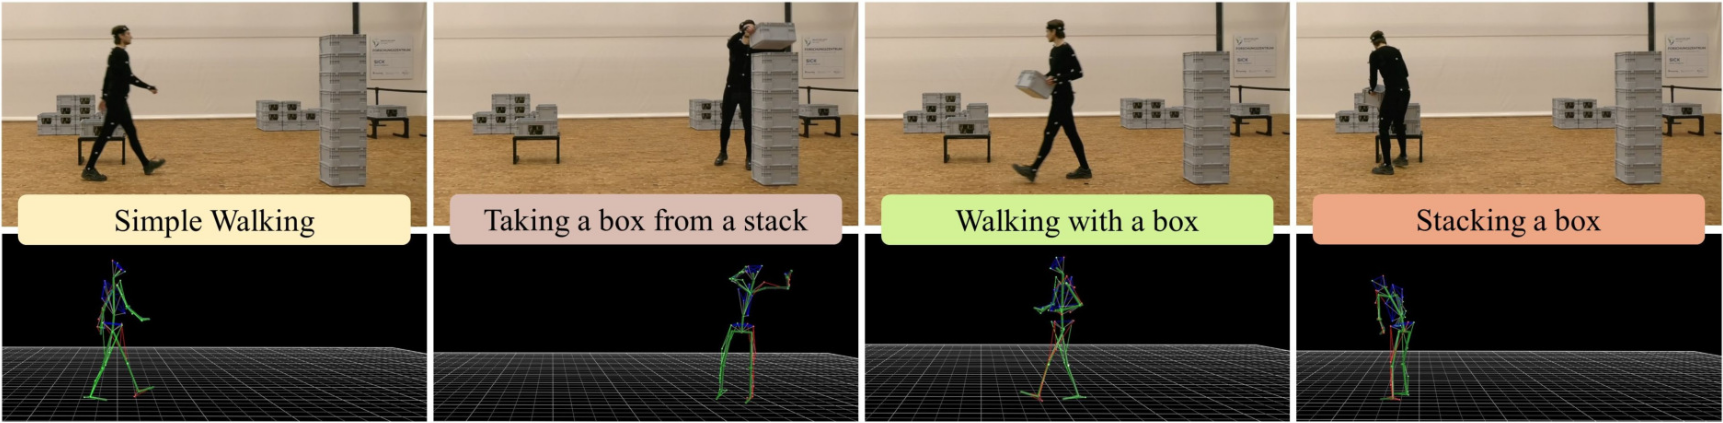
\includegraphics[width=\textwidth]{har-image-skeleton.png}
    \caption{Example of human acitivies in a warehouse context. Taken from \fcite{reining_towards_2018}}
  \end{figure}
\end{myframe}

\tableofcontents

\section{Fundamentals}
\subsection{Human Activity Recognition}

\section{Related Work}
\subsection{2D / 3D pose estimation}

\begin{myframe}[2D pose estimation]
  \begin{itemize}
    \item \textbf{shallow methods}
    \begin{itemize}
      \item Mixture-of-parts model \fcite{yang_articulated_2011}
    \end{itemize}
    \item \textbf{deep methods}
    \begin{itemize}
      \item Stacked hourglass \fcite{newell_stacked_2016}
      \item Convolutional pose machine \fcite{wei_convolutional_2016}
    \end{itemize}
  \end{itemize}
\end{myframe}

\subsection{Video-based HAR}
% For Joint estimation AND HAR
%   Shallow methods 
%   Deep Learning

\section{Method}

\section{Datasets}
% also: metrics?

\section{Conclusion}
%also: Vielen Dank slide

\begin{myframe}[Eine Folie mit Referenzen]
Der Einfachheit halber zitiere ich mich einmal selbst \fcite{wang_approach_2013}
und gleich nochmal \fcite{yang_articulated_2011}.
\vspace*{3ex}

Hinweis: bibtex ggf. von Hand zwischendurch aufrufen, wenn mal Referenzen fehlen.
 
\end{myframe}

% \begin{myframe}[Eine komlexere Folie mit Referenzen]
% Wenn man etwas Spezielleres will, z.b. etwas zitieren
% \footnotetext[1]{\bibentry{Bauer2012}}\footnotemark[1] 
% was anderes \footnotetext[2]{\bibentry{Plinge2010-RNF}}\footnotemark[2] 
% und auf derselben Folie später dasselbe nochmal, 
% \footnotemark[1]
% muss man leider etwas basteln...
% \end{myframe}


\end{document}

